\documentclass[a4paper,12pt,fleqn]{article}
\usepackage{fixltx2e}
\usepackage[utf8]{inputenc}
\usepackage{graphicx}
\usepackage{sidecap}
\usepackage{fancyhdr}
\usepackage{amssymb,amsmath}
\usepackage[swedish]{babel}
\usepackage[margin=1.5in]{geometry}
\usepackage{abstract}
\usepackage[parfill]{parskip}
\usepackage{tocloft}
\usepackage{adjustbox}
\usepackage{textcomp}
\usepackage[T1]{fontenc}
\usepackage[usenames,dvipsnames,svgnames,table]{xcolor}
\usepackage{listings}
\usepackage{hyperref}
\usepackage{tocloft}
\usepackage{mathpazo}

% %% Footnotes-Listing %%
\newcommand{\listfootnotesname}{Referenser}% 'List of Footnotes' title 
\newlistof[chapter]{footnotes}{fnt}{\listfootnotesname}% New 'List of...' for footnotes 
\let\oldfootnote\footnote % Save the old \footnote{...} command 
 \renewcommand\footnote[1]{% Redefine the new footnote to also add 'List of Footnote' entries. 
     \refstepcounter{footnotes}% Add and step a reference to the footnote/counter. 
     \oldfootnote{#1}% Make a regular footnote. 
     \addcontentsline{fnt}{footnotes}{\protect 
 \numberline{\thefootnotes}#1}% Add the 'List of...' entry. 
}

%----------------------------------------------------------------
%C-kod formatering

\definecolor{listinggray}{gray}{0.9}
\definecolor{lbcolor}{rgb}{0.9,0.9,0.9}
\lstset{
backgroundcolor=\color{lbcolor},
    tabsize=4,    
%   rulecolor=,
    language=[GNU]C++,
        basicstyle=\scriptsize,
        upquote=true,
        aboveskip={1.5\baselineskip},
        columns=fixed,
        showstringspaces=false,
        extendedchars=false,
        breaklines=true,
        prebreak = \raisebox{0ex}[0ex][0ex]{\ensuremath{\hookleftarrow}},
        frame=single,
        numbers=left,
        showtabs=false,
        showspaces=false,
        showstringspaces=false,
        identifierstyle=\ttfamily,
        keywordstyle=\color[rgb]{0,0,1},
        commentstyle=\color[rgb]{0.026,0.112,0.095},
        stringstyle=\color[rgb]{0.627,0.126,0.941},
        numberstyle=\color[rgb]{0.205, 0.142, 0.73},
%        \lstdefinestyle{C++}{language=C++,style=numbers}’.
}
\lstset{
    backgroundcolor=\color{lbcolor},
    tabsize=4,
  language=C++,
  captionpos=b,
  tabsize=3,
  frame=lines,
  numbers=left,
  numberstyle=\tiny,
  numbersep=5pt,
  breaklines=true,
  showstringspaces=false,
  basicstyle=\footnotesize,
%  identifierstyle=\color{magenta},
  keywordstyle=\color[rgb]{0,0,1},
  commentstyle=\color{Darkgreen},
  stringstyle=\color{red}
  }
  %-----------------------------------------------------------------
  %marginaler

  \renewcommand{\abstractnamefont}{\normalfont\normalsize\bfseries}
  \renewcommand{\abstracttextfont}{\normalfont\small}
  \renewcommand{\headrulewidth}{0pt}
  \renewcommand{\cftsecleader}{\cftdotfill{\cftdotsep}} 
  \setlength{\absleftindent}{0pt}
  \setlength{\absrightindent}{0pt}
  \setlength{\headheight}{15pt}

  \addtolength{\oddsidemargin}{-.5in}
  	\addtolength{\evensidemargin}{-.5in}
  	\addtolength{\textwidth}{1in}


  %-----------------------------------------------------------------
  %header and footer

  \pagestyle{fancy}
  \lhead{
  	\begin{picture}(0,0)
  		\put(5,0){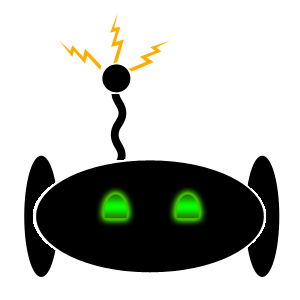
\includegraphics{logotyp.png}}
  	\end{picture}}
	
  \fancyhead[C]{\small{Mapmaster2001}}
  \fancyhead[R]{\small \today}
  \fancyfoot[L]{\small{TSEA56 \\ LIPS Kappa}}
  \fancyfoot[C]{\small{\thepage}}
  \fancyfoot[R]{\small{Projektgrupp 8 \\ mapmaster2001@cyd.liu.se}}

  %-----------------------------------------------------------------


%-------------------------------------------------------------------
%Första sidan
\begin{document}
	\pagestyle{empty}
\pagenumbering{gobble}
	\vspace*{\fill}
		\begingroup
			\begin{center}
				\huge{\textbf{Efterstudie}}
				\\
				\vspace{5pt}
				\normalsize
				Kandidatprojekt Y - Grupp 8 - VT2014
				\\
				Version 1.0
				\end{center}
		\endgroup
	 
	\vspace{15pt}
	\vspace*{\fill}
	
	\begin{center} %Börjar centrering 
		Status
		\\
		\vspace{3pt} %Whitespace 3 pts
	    \begin{tabular}{| p{3cm} | p{3cm} | p{3cm} |} %tabell, 4 horizontella |, 3 cm emellan dem.
	    \hline %översta horizontella linjen.
	    Granskad & JE,TG,HFE & \today \\ \hline % & -tecken för att "gå till nästa ruta" 
		Godkänd & - & - \\ \hline % avslutas med \\ och \hline.

	    \end{tabular}
	\end{center}
	\vspace{2cm}
	\newpage
%-----------------------------------------------------------------
%Projektidentitet
	
	\vspace*{\fill}
		\begingroup
			\begin{center}
				\LARGE{\textbf{PROJEKTIDENTITET}}
				\\
				\footnotesize
				Grupp 8, 2014/VT, MapMaster2001
				\\
				Linköpings tekniska högskola, ISY
				\\
				\vspace{1cm}
	  \begin{tabular}{| p{3cm} | p{4.3cm} | p{2.4cm} | p{3.8cm} |}
	    \hline
		\textbf{Namn} & \textbf{Ansvar} & \textbf{Telefon} & \textbf{E-post} \\ \hline
	    Jens Edhammer & Dokumentansvarig (DOK) & 076-030 67 80 & jened502@student.liu.se \\ \hline
		Erik Ekelund & Designansvarig (DES) & 073-682 43 06 & eriek984@student.liu.se \\ \hline
		David Habrman &  & 076-017 71 15 & davha227@student.liu.se \\ \hline 
		Tobias Grundström & Testansvarig (TES) & 073-830 44 45 & tobgr602@student.liu.se \\ \hline 
		Hans-Filip Elo &   & 073-385 22 32 & hanel742@student.liu.se \\ \hline 
		Niklas Ericson & Projektledare (PL) & 073-052 27 05 & niker917@student.liu.se \\ \hline
	    \end{tabular}
		
		\vspace{1cm}
		\textbf{E-postlista för hela gruppen:} mapmaster2001@cyd.liu.se
		\\[0.5cm]
		
		\textbf{Kund}: Mattias Krysander, Linköpings universitet, 581 83  LINKÖPING, \\
		013-28 21 98, matkr@isy.liu.se \\
		\textbf{Kontaktperson hos kund}: Mattias Krysander, 013-28 21 98, matkr@isy.liu.se 
		\\
		\textbf{Kursansvarig}: Tomas Svensson, 3B:528,013 28 21 59, tomass@isy.liu.se
		\\[0.5cm]
		\textbf{Handledare}: Peter Johansson, 013-28 1345, peter.a.johansson@liu.se

				\end{center}
		\endgroup
	\vspace*{\fill}
\newpage

%-----------------------------------------------------------------
%Innehållsföreteckning

\addto\captionsswedish{\renewcommand{\contentsname}{Innehållsförteckning}}

\tableofcontents
\newpage
\pagestyle{fancy}
\pagenumbering{arabic}

%-----------------------------------------------------------------
%Översikt

\section{Tidsåtgång}
Generellt sett har projektet tagit lite längre tid än planerat men inte mycket. I Under-fasen la vi ner 1525 timmar totalt men vi hade bara budgeterat för 1380 timmar. Det som framför allt framgick tydligt efter en bit in i projektet var att många av aktiviteterna var onödiga eller gick i varandra. Det är dock inte så konstigt att det blev på det här viset med tanke på att vi i För-fasen inte hade en aning om hur saker och ting skulle utföras eller hur lång tid det skulle ta. 

\subsection{Arbetsfördelning}
Arbetsfördelning under projektet har varit god. Vi har alltid försökt eftersträva att man ska kunna jobba parallellt med varandra med olika uppgifter. Detta har självklart inte alltid gått att genomföra då vi endast har haft en robot, men i många fall har vi kunnat jobba med saker på sidan om. I en fas i projektet hade vi till och med två stycken virkort som var identiskt virade för att kunna testa bluetooth på det ena och display på den andra. Arbetet har oftast skett i par och varje par har haft en ansvarsområde. I början av projektet delades gruppen upp i tre och varje delgrupp tog varsin modul. När roboten i ett senare stadie i projektet var monterad splittrades grupperna upp och nya par bildades. På det här sättet spred vi ut kunskapen kring modulerna i gruppen. 

\newpage
\subsection{Tidsåtgång jämfört med planerad tid}
I figur~\ref{fig:tid} syns klart och tydligt att vi försökt följa den ursprungliga planen från början men att det på slutet arbetades en del över budget. Detta beror på att vi i slutet hade en rad olika problem med bussen som tog en massa tid från projektet. När problemet med bussen var hyfsat löst återstod bara 2 dagar innan leverans och vi var tvungna att skriva kartsökningsalgoritmen väldigt snabbt. Vi la också ner väldigt mycket tid på en Astar-algoritm som visade sig vara okörbar på Atmega 1284p. 

\begin{figure}[htp] %Placera här om det finns plats, annars så snart som möjligt, på toppen av en sida.
  \begin{center}
  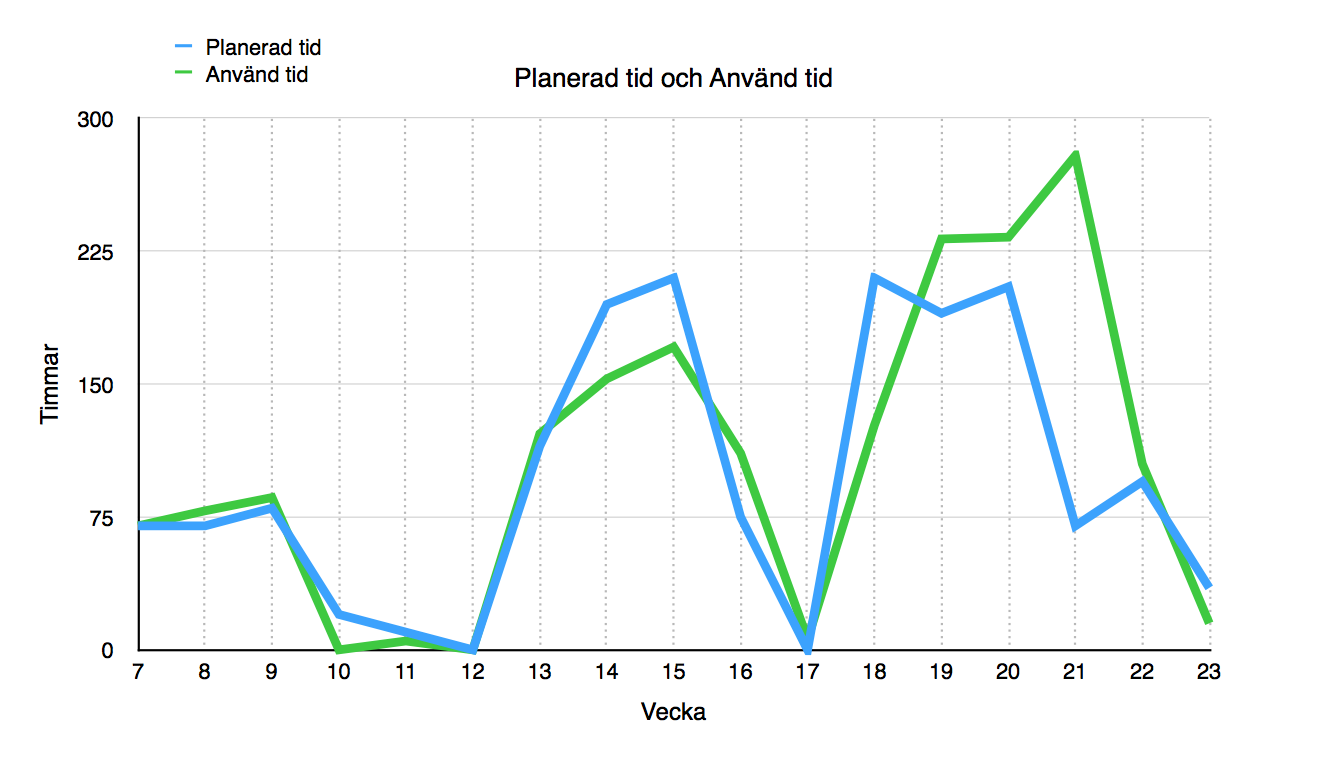
\includegraphics[keepaspectratio=true,scale=0.25]{tid.png}  %skala och filnamn. 
  \end{center}
  \caption{Diagram över planerad och använd tid} %figurtext.
  \label{fig:tid}
\end{figure}

\newpage

\section{Analys av arbete och problem}
Arbetet i projektet har sånär som på ett par veckor flutit på bra och projektmodellen har följts överlag. De veckor som inte fungerade lika bra som övriga berodde till stor del på tekniska problem.

\subsection{Vad hände under de olika faserna (bra/dåligt/orsak)}
%%Jag fattar inte vad vi ska skriva här? :S
Då krav- och designspecifikationer skrevs var det svårt att se hur man skulle lösa vissa problem i projektet - och även hur lång tid många delar av projektet skulle förbruka. Det brukar kännas som en naturlig del i projektstyrning - det ska helt enkelt vara svårt att planera arbetet på förhand. 

I underfasen påbörjades arbetet med designspecifikationen följt av att arbetet i muxen och fördjupningsuppgift. Ett problem här är att fördjupningen borde ha tillhört förefasen för att få ut så mycket som möjligt av den. En sak i underfasen som vi själva borde jobbat mer med är tester. Gruppen fick ett väldigt resultatsinriktad inställning och i slutet av projektet när tiden blev knapp var det en del tester som det helt enkelt inte fanns tid till att utföra. Underfasen avslutades med att roboten presenterades för beställare som godkände produkten i dess befintliga skick. 

I efterfasen utfördes en presentation för en av de andra grupperna och för beställaren. Denna fas blev inte så lyckad som man kanske velat då efterfasen låg mitt i tentaperioden. Tentaperioden överlappade även till viss del med underfasen - vilket inte heller kändes optimalt. 


\subsection{Hur arbetade vi tillsammans}
I början av varje vecka hölls ett kortare möte där veckans arbete diskuterades och mindre delgrupper skapades på aktivitetsnivå. Dessa grupper skiftade emellanåt då nya problem eller aktiviteter uppstod. De personer som arbetade med ett givet problem fick även ansvar för att meddela resterande av gruppen om mer resurser behövdes eller om nya problem uppstod. Kommunikation sköttes löpande mellan delgrupperna då man ofta utnyttjade varandra som bollplank i felsökning eller hade löst någonting som man tyckte var häftigt och därför ville berätta. Kommunikation blev helt enkelt väldigt organisk och behövdes inte styras. 
Inför alla större beslut kallades det till möte med samtliga projektmedlemmar.

Samtliga medlemmar i gruppen har hög ambitionsnivå och är stundtals envisa, det var därför inte helt ovanligt att ibland kunna hitta oss argumentera kraftigt med varandra. Detta är något vi vet om att vi gör sedan tidigare projekt tillsammans. Det har aldrig varit ett problem och vi känner inte att det har varit ett problem nu heller. Vi blir helt enkelt vänner igen när dagen är slut. 

\subsection{Hur använde vi projektmodellen}
Vi har genom hela projektet utgått från projektmodellen. Det som varit svårast med modellen är att försöka följa den första tidsplanen, istället har denna uppdaterats efterhand. I början av varje vecka har vi på ett mindre möte kollat över vilka aktiviteter som vi tycker borde ha mer/mindre tid under kommande vecka. I och med att gruppen redan arbetat ihop i tidigare projekt, och att alla i projektgruppen har en väldigt hög ambitionsnivå, vet vi vad vi kan förvänta av varandra. Vi fann därför att projektmodellen med på förhand specificerad tid per aktivitet (istället för enbart milstolpar att nå) blev väldigt redundant och inte till ett egentligt hjälpmedel. 

\subsection{Hur fungerade relationen med beställaren?}
Relation med beställaren har varit problemfri. Han svarar alltid snabbt på mail, verkar genuint intresserad och har alltid konstruktiv kritik att komma med. Han verkar också uppskattat de lösningar vi skapat rent tekniskt. Hela gruppen har haft ett väldigt kul och bra samarbete med vår beställare. 

\subsection{Hur fungerade relationen med handledaren?}
Ibland kunde vår handledare vara svår att nå, dock endast i början av projektet. Det märktes tidigt att det krävdes en välformulerad och riktad fråga för att få ett bra svar, detta är självklart inga konstigheter och har istället hjälpt oss under projektet då en del fel löste sig genom att gruppen tänkte igenom frågor i detalj i förväg. I slutet av projektet var handledaren mycket lättare att nå och komma ofta förbi labbet för att kolla till sina grupper och deras status. Det märktes tydligt att handledaren var mycket kunnig och vi är mycket nöjda med handledaren.

\subsection{Tekniska problem}

Hårdvaru- och mjukvarufel som gjorde att moduler startade om. 
Vid ett tillfälle i robotens konstruktion stötte vi på bussproblem. Kommunikation kom inte över korrekt. Vi började felsöka detta och fann till slut orsakerna. Det visade sig vara flera parallella problem som gav liknande symptom. En trasig anslutning till robotens chassi gjorde att modulen emellanåt startade om p g a spänningsfall. Modulen startade om sig p g a att en dålig implementering av en kopiering utnyttjade för mycket minne och processorns programpekare slog om i programmet. Dessutom hade vi en trasig processor som också hade beteendet att den startade om. Detta problem fanns sporadiskt över 2 veckor innan det fullständigt löstes. Vi förlorade nog inte de hela 2 veckorna på felen då annat byggdes parallellt, men vi förlorade säkerligen 1 - 1,5 vecka.

Mjukvarufel i implementering av någon funktion resulterade i att bussen inte fungerade korrekt utan kunde ibland låsa sig.
Felsökningen gav inga resultat och vi fick tillslut rulla tillbaka vår kod tills när den senast fungerade, sex dagar tidigare. Detta blev ett stort steg bakåt och uppskattningsvis förlorade vi 8 dagar.

Otillräcklig noggrannhet i sensorer ledde till att designval var tvungna att ändras.
Vi insåg efter ett tag att avståndsbestämning med långdistanssensorerna inte skulle fungera med tillräckligt hög precision. Sensorerna var för brusiga vid långa distanser och kunde emellanåt slå i en vägg. Vi ändrade metoden för distansmätning till reflexsensorn som mäter hjulets rotation. Detta fungerade väldigt bra och var väl värd tiden vi förlorade på att implementera om avståndsmätningen. På detta fel förlorade vi ungefär 2 dagar.

\subsection{Tekniska framgångar}
Vi är otroligt nöjda med våra rotationer vilka blev väldigt precisa.
Dessa löstes med ett analogt gyro och om möjligt så är det så vi skulle implementera det igen. Dessutom blev avståndmätningarna med hjälp av reflexsensorerna väldigt bra och på en sex meter lång sträcka hade vi en felmarginal på mindre än $\pm$10 cm. Avståndsgraferna och kartan i vårt GUI blev bra och kunde användas för felsökning vilket underlättade mycket under hela projektets gång. 

\section{Måluppfyllelse}
Gruppen hade som initialt mål att leverera produkt med uppfyllda krav 1 mål samt att genomföra ett välarbetat och professionellt projekt. Detta tycker vi har uppfyllts, även om kravbilden omförhandlats under projektets gång. 

\subsection{Vad har uppnåtts?}
I dagsläget finns en robot som autonomt kartlägger ett slutet område med köksöar inuti. Den kan även detektera RFID-taggar, dock har vi haft problem med hårdvaran för RFID-avläsning, så denna fungerar . 

\subsection{Hur fungerade leveransen?}
Leveransen skedde genom ett möte med beställare där produkten demonstrerades genom en serie av körningar i olika typer av banor. Övriga funktioner såsom manuell styrning och kartlagring visades också upp. Kravlistan gicks igenom ett krav i taget och verifierades om målet var uppnått eller ej. I slutet av mötet tog beställare beslut om produkten var färdigställd. Vi är mycket nöjda med leveransen både i utformning och resultat.

\subsection{Hur har studiesituationen påverkat projektet?}
Om möjligt skulle, inte bara för vår skull men även för andra examinatorer, projektkursen hållas enskilt utan övriga kurser parallellt. De flesta studenter  väljer att prioritera projektet över andra kurser då projektkursen är på 16hp och skulle vara förödande att förlora dessa. 

Stor arbetsbörda med fördjupningsuppgiften som ingår i projektet har också sinkat några av gruppens medlemmar - både i sin prestation i projektet och även i andra kurser. Specificerade tiden 50 timmar har inte varit tillräckligt för dem där. 

\section{Sammanfattning}
\subsection{De tre viktigaste erfarenheterna}

Att oscilloskopet är ett bra verktyg har vi alltid förstått, men under projektets gång insåg vi hur viktigt det var vid felsökning av hårdvara och hårdvarunära mjukvaruimplementeringar. Oscilloskopet underlättade analys av flera signaler parallellt vilket gjorde det möjligt att bland annat se hur data skickades ut på bussen, inte bara hur den togs emot.

Vi har lärt oss att det är svårt att implementera en buss. Hade vi fått göra om projektet hade vi valt att använda en starkare huvudprocessor gör att hantera sensordata och ta vägvalsbeslut. En starkare processor av en annan arkitektur (ex ARM) kan också använda högnivåbibliotek vilka markant förbättrar möjligheterna till att skapa avancerade kartläggnings och vägfinnaralgoritmer. 

\subsection{Goda råd till de som ska utföra ett liknande projekt}
Det första rådet vi har till de som ska utföra ett liknande projekt är att planera noga och att fördela antalet arbetstimmar jämnt över hela projektettiden. En bra och tydlig planering är viktigt och kommer underlätta allt arbete. Att fördela arbetstimmarna jämnt över veckorna gör det lättare att lägga mer tid på andra kurser som läses parallellt med kandidatprojektet.

Det är också viktigt att lägga mycket tid på utveckling av bussprotokoll, men framförallt test av buss i början av projektet. Att testa bussen noggrant har man igen senare i projektet. Bussen kan med fördel testas mycket och med olika fall för att se att allt fungerar som det ska. Vi insåg i slutet av arbetet att vår buss inte var byggd på en tillräckligt bra implementering, men då var det för sent för att göra något åt det.

\end{document}
